\documentclass[12pt]{article}
\usepackage{parskip,amsmath,enumitem,graphicx}
\usepackage[margin=.6in]{geometry}
\usepackage{color}
\newcommand{\hilight}[1]{\colorbox{yellow}{#1}}
\begin{document}
\title{Assignment 2}
\maketitle
\author{Lara Janecka, lajaneck, 20460089}
\subsection*{Ch5: q44}
A man had to have the muffler replaced on his two-year-old car. The repairman offered two alternatives. For \$300 he would install a muffler guaranteed for two years. For \$400 he would install a muffler guaranteed ``for as long as you own the car''. Assuming the present owner expects to keep the car for about three more years, which muffler would you advise him to have installed if you thought 20\% was a suitable interest rate and the less expensive muffler would only last two years.

\begin{align*}
    PW_a &= -300 - 300(P/F, 20\%, 2)\\
         &= -300 - 300(.6944)\\
         &= -508.32\\
    PW_b &= -400
\end{align*}

Since the present value of buying the more expensive muffler is better I advise him to buy \\\hilight{the more expensive muffler}.

\subsection*{Ch5: q75}
The following coses are associated with three tomato-peeling machines being considered for use in a canning plant. If the canning company uses an interest rate of 12\%, which is the best alternative? Use NPW to make your decision.\\
\begin{center}
\begin{tabular} {| c | c c c|}
\hline
 & \textbf{Machine A} & \textbf{Machine B} & \textbf{Machine C}\\
\hline
First cost & \$52,000 & \$63,000 & \$67,000\\
Maintence and Operation cost & \$15,000 & \$9,000 & \$12,000\\
Annual benifit & \$38,000 & \$31,000 & \$37,000\\
Salvage value & \$13,000 & \$19,000 & \$22,000\\
Useful life & 4 & 6 & 12\\
\hline
\end{tabular}
\end{center}

\begin{align*}
NPW_A &= -52000 + (13000 - 52000)(P/F, 12\%, 4) + (13000 - 52000)(P/F, 12\%, 8) + 13000(P/F, 12\%, 12)\\
      &+ (38000- 15000)(P/A, 12\%, 12)\\
      &= -52000 + (13000 - 52000)(.6355) + (13000 - 52000)(.4039) + 13000(.2567)\\
      &+ (38000- 15000)(6.194)\\
      &=\$53,262.50\\
NPW_B &= -63000 + (19000 - 63000)(P/F, 12\%, 6) + 19000(P/F, 12\%, 12)\\
      &+ (31000- 9000)(P/A, 12\%, 12)\\
      &= -63000 + (19000 - 63000)(.5066) + 19000(.2567)\\
      &+ (31000- 9000)(6.194)\\
      &=\$55,854.90\\
NPW_C &= -67000\\
      &+ (37000-12000)(P/A, 12\%, 12)\\
      &+ 22000(P/F, 12\%, 12)\\
      &= -67000\\
      &+ (37000-12000)(6.194)\\
      &+ 22000(.2567)\\
      &= 93497.40
\end{align*}

Since it has the highest NPW chose \hilight{Machine C}.

\subsection*{Ch6: q37}
Jenny McCarthy is an engineer for a municipal power plant. The plant uses natural gas, which is currently obtained from an existing pipeline at an annual cost of \$10,000 per year. Jenny is considering a project to construct  a new pipeline. The initial cost of the new pipeline would be \$35,000, but it would reduce the annual cost to \$5,000 per year. Assuming an analysis period of 20 years and no salvage value for either the existing or new pipeline. The interest rate is 6\%.\\
(a) Determine the equivalent uniform annual cost for the new pipeline.\\
\begin{align*}
EUAC &= 35000(A/P, 6\%, 20) + 5000\\
    &= 35000(.0872) + 5000\\
    &= 8052
\end{align*}
Since \hilight{\$8,052} is less than the EUAC of the current pipeline you should \hilight{build the new one}.

\subsection*{Ch6: q48}
Which car has the lower EUAC if the owner can earn 5\% in his best investment?
\begin{center}

\begin{tabular}{c | c c}
\hline
 &\textbf{Toyota Corolla} & \textbf{Toyota Prius}\\
 \hline
Iniital cost & 19200 & 25500\\
Annual maintenence & 1000 & 1500\\
Annual gas \& oil (increasing 15\% yearly) & 2500 & 1200\\
Salvag/e value (EOY8) & 8000 & 10000\\
\hline
\end{tabular}
\end{center}
\begin{align*}
EUAC_{Corolla} &= 19200(A/P, 5\%, 8) + 1000 + 2500(P/G, 15\%, 5\%, 8) - 8000(A/F, 5\%, 8) \\
    &= 19200(.1547) + 1000 + 2500(.0934) - 8000(.1047)\\
    &= 3366.14\\
EUAC_{Prius} &= 25500(A/P, 5\%, 8) + 1500 + 1200(P/G, 15\%, 5\%, 8) - 10000(A/F, 5\%, 8) \\
    &= 25500(.1547) + 1500 + 1200(.0934) - 10000(.1047)\\
    &= 4509.93
\end{align*}
Since the prius has a higher equivalent annual cost \hilight{chose the Toyota Corolla}.

\subsection*{Ch6: q58}
Consider the following alternatives:\\
\begin{center}

\begin{tabular}{|c | c c|}
\hline
& \textbf{A} & \textbf{B}\\
\hline
Cost & 5000 & 18000\\
Uniform annual benefit & 1500 & 6000\\
Useful life &10 & 5\\
\hline
\end{tabular}
\end{center}

The analysis period is 10 years, but there will be no replacement for Alternative B after five years. Assuming a 15\% interest rate, decide which alternative should be chosen. Use an annual cash flow analysis.

\begin{align*}
EUAC_A &= 5000(P/A, 15\%, 10) - 1500\\
    &= 5000(.1993) - 1500\\
    &= -503.5\\
EUAC_B &= 18000(P/A, 15\%, 5) - 6000\\
    &= 18000(.2310) - 6000\\
    &= -1842
\end{align*}

Since option B has a lower equivalent annual cost \hilight{chose option B}.

\subsection*{Ch6: q64}
A student loan total \$18,000 at graduation. The interest rate is 6\%, and there will be 60 payments beginning one month after graduation. What is the monthly payment? What is owed after the first two years of payments? Use a spreadsheet.
\begin{center}

\begin{tabular}{| c | c | c |}
\hline
& A & B\\
\hline
1 & 18000 & initial balance\\
\hline
2 & 0.5\% & nominal interest\\
\hline
3 & \$347.99 & -PMT(A2,A3,A1)\\
\hline
\end{tabular}
\end{center}

\subsection*{Q1}
Bill wants to have a car during his college year (5 years), and has two options. He can
lease a car with \$4,000 of down payment (which is not refundable), \$1,000 of security deposit (fully refundable), and \$500 of monthly payment for 5 years. Alternatively, he can buy a car for \$30,000 now and sell it 5 years later. What is the minimum salvage value of the car that makes buying preferable, assuming an interest rate of 12\%?
\begin{align*}
-5000 + 1000(P/F, 1\%, 60) - 500(P/A, 1\%, 60) &= -30000 + X(P/F, 1\%, 60)\\
-5000 + 1000(.5504) - 500(44.955) &= -30000 + X(.5504)\\
X &=5583.03
\end{align*}

Bill needs to salvage the car for at least \hilight{\$5,583.03}.

\subsection*{Q2}
Compute the present worth of the following cash flows, given an interest rate of 6\%.
\begin{center}
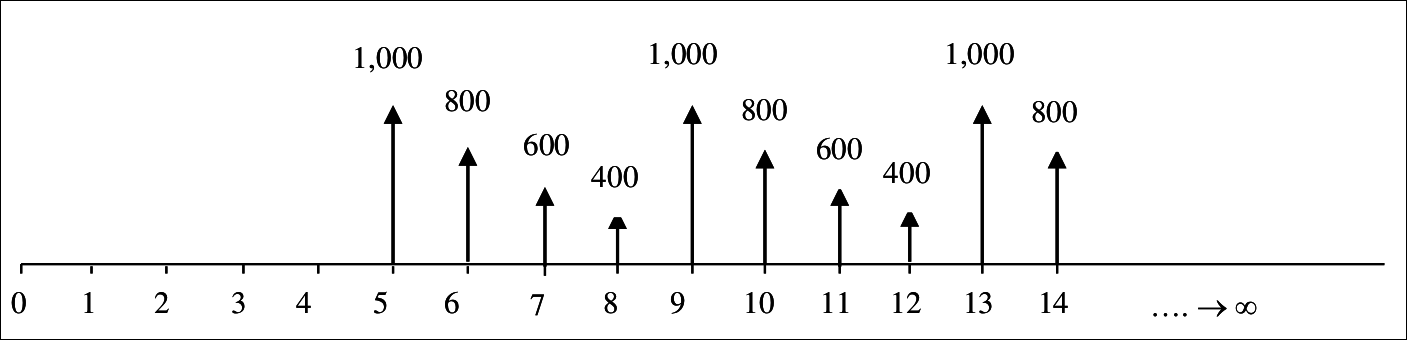
\includegraphics[width=15cm]{q2.png}
\end{center}
\begin{align*}
A_{yearly} &= 400 + 200(A/G, 6\%, 4)\\
&= 400 + 200(1.427)\\
&= 685.4\\
P_5 &= \frac{A_{yearly}}{i}\\
&= \frac{685.4}{0.06}\\
&=11423.33\\
P&=11423.33(P/F, 6\%, 5)\\
&=11423.33(.7473)\\
&=8536.66
\end{align*}

The present worth of the cash flow is \hilight{\$8,536.66}

\subsection*{Q3}
A new machine costs \$700,000 and will bring net benefits of \$100,000 for its first 6
years of operation. Thereafter, these net benefits will be reduced by 8\% per year due to increases in maintenance costs (e.g., the net benefit in the 7th year is \$94,600, and so on). The expected service life of the machine is 15 years and its salvage value at the end of the 15th year is \$40,000. Assuming an interest rate of 6\%, what is the annual worth of using the robot? Draw the cash flow diagram first.
\begin{center}
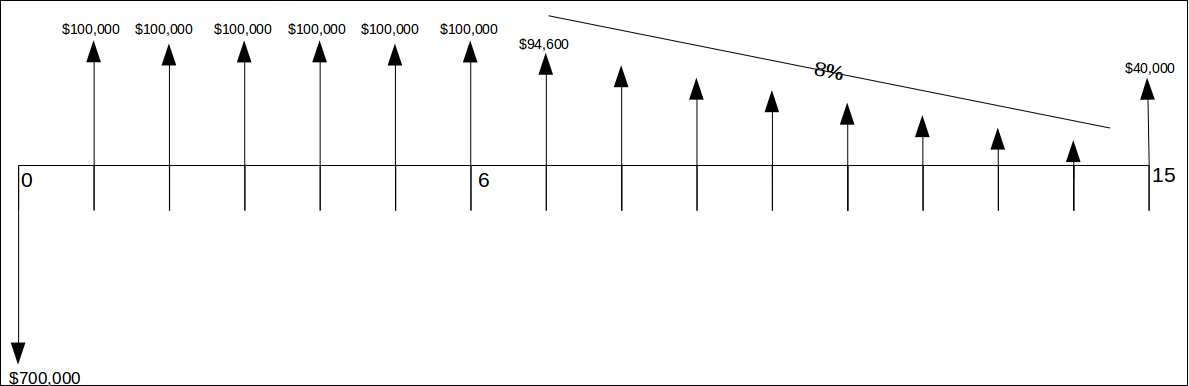
\includegraphics[width=15cm]{q3.png}
\end{center}

\begin{align*}
P_1 &= 100000(P/A, 6\%, 6)\\
&= 100000(4.917)\\
&= 491700\\
P_2 &= 100000(P/G, -8\%, 6\%, 9)\\
&=100000(5.961)\\
&=596100\\
P &= -700000 + P_1 + P_2(P/F, 6\%, 6) + 40000(P/F, 6\%, 15)\\
&= 491700 + 596100(.7050) + 40000(.4173)\\
&= 228642.50\\
EUAW &= P(A/P, 6\%, 15)\\
&=228642.50(.103)\\
&=23550.18
\end{align*}
The annual worth of the machine is \hilight{\$23,550.18}.

\subsection*{Q4}
A local car dealer offers “zero percent” interest on a \$30,000 automobile for 48
monthly payments. If a customer either pays cash or makes other financing arrangements, there is a discount of \$4,000 from the car company. An Engineering Economics professor at UW argues that instead of using the dealer’s zero percent loan, you should take loan at 6\% for 4 years from a credit union considering \$4,000 rebate. Is he right?

\begin{align*}
EUAC_{dealer} &= \frac{30000}{48}*12\\
&= 7500\\
EUAC_{prof} &= 26000(A/P, 6\%, 6)\\
&= 26000(.2886)\\
&= 7503.6
\end{align*}
 Since the proffessors plan results in a higher annual cost you should take the \hilight{dealer's option}.

\subsection*{Q5-8}
As soon as he got a job, John decided to open a savings account for his retirement. The account is expected to pay 12\% interest rate, compounded quarterly. John wishes to save \$500,000 at the end of 25 years. Calculate the annuity if it is paid at:

\subsection*{Q5}
the end of each quarter.

\begin{align*}
i_e &= (1 + .12)^{\frac{1}{4}} - 1\\
&= 0.0287\\
A &= 500000(A/F, 2.87\%, 4*25)\\
&= 500000(.00165)\\
& 825
\end{align*}

\hilight{annuity = 825}

\subsection*{Q6}
the end of each month.

\begin{align*}
i_e &= (1 + .12)^{\frac{1}{12}} - 1\\
&= .00095\\
A &= 500000(A/F, 0.95\%, 12*25)\\
&=500000\bigg ( \frac{.0095}{(1.0095^{300})-1} \bigg)\\
&=295.83
\end{align*}

\hilight{annuity = 295.83}

\subsection*{Q7}
at the end of each year.

\begin{align*}
i_e &= .12\\
A &= 500000(A/F, 12\%, 25)\\
&= 500000(.00750)\\
&= 3750
\end{align*}

\hilight{annuity = 3,750}

\subsection*{Q8}
at the beginning of each year.

\begin{align*}
i_e &= .12\\
A &= 500000(A/F, 12\%, 26)\\
&= 500000(.00665)\\
&= 3325
\end{align*}
\hilight{annuity = 3,325}

\subsection*{Q9}
Joe bought a BMW when he came to UW as an engineering student, by taking a loan
that was to be paid off in 20 equal, quarterly payments. The interest rate on the loan was 12\% per year with quarterly compounding. After four years, at the time that Joe made his 16th payment, he sold the BMW to his buddy Sam. Sam made arrangements with Joe's bank to refinance the loan and to pay Joe's unpaid balance by making 16 equal quarterly payments at the same interest rate that Joe was paying. After 3 and 1⁄4
years, at the time that Sam made his 13th payment, Sam sold the car to Nancy.
Nancy paid the bank \$2,000 cash to pay the loan balance. What was the amount of Joe's loan to purchase the BMW when it was new?

\begin{align*}
Sam_A &= 2000(A/P, 3\%, 3)\\
&=2000(.3535)\\
&= 707\\
Sam_P &= 707(P/A, 3\%, 13)\\
&= 707(10.635)\\
&= 7518.945\\
Joe_P &= 7518.945(P/F, 3\%, 16)\\
&= 7518.945(.6232)\\
&=4685.81
\end{align*}

Joe's initial loan was \hilight{\$4,685.81}.

\subsection*{Q10}
A magazine offers life-time subscription for \$200. Such a subscription may be given
as a gift to an infant at birth (the parents can read it in those early years) or taken out by an individual for himself. The magazine costs \$12.90 a year. This price is expected to be constant. What rate of return would the parents obtain if they bought a life subscription rather than paying \$12.90 per year beginning immediately? You may make any reasonable assumptions, but the compound interest factors must be used correctly. (If you cannot find the exact rate, please find the range of the rates.)

Assume that the child will live for 100 years.
\begin{align*}
200 &= 12.9(P/A, i, 100)\\
15.5 &= (P/A, i, 100)\\
i &= \text{ between 6 and 7}
\end{align*}

The rate of return is \hilight{between 6\% and 7\%}





\end{document}
